\subsection{fbwarn}
Falls die Festplattenverifizierung Fehlschlägt, muss der Nutzer gewarnt werden (es ist auch möglich das Gerät einfach auszuschalten, jedoch sollte dies aus UX gründen nicht gemacht werden).

\subsubsection{Grafischer Output}
Die Warnung ist am besten grafisch zu tun, jedoch gibt es keinen display server wie Wayland oder X11, deshalb muss direkt auf den Framebuffer /dev/fb* geschrieben werden, um graphischen Output zu zeigen.\\
Da jeder verfügbare framebuffer als /dev/fbX verfügbar ist, kann man ganz einfach die Datei öffnen und mit mmap manipulieren:

\begin{minted}[fontsize=\footnotesize]{c}
 // imports: stdlib, linux/fb.h, stdio
 int main()
 {
     int fbfd = 0;
     struct fb_var_screeninfo vinfo;
     struct fb_fix_screeninfo finfo;
     
     // Open the framebuffer file for reading and writing
     fbfd = open("/dev/fb0", O_RDWR);
          
     // Get fixed screen information
     ioctl(fbfd, FBIOGET_FSCREENINFO, &finfo);
     // Get variable screen information
     ioctl(fbfd, FBIOGET_VSCREENINFO, &vinfo);
  
     // Map the device to memory
     fbp = (char *)mmap(0, screensize, PROT_READ | PROT_WRITE, MAP_SHARED, fbfd, 0);
 
     location = (300+vinfo.xoffset) * (vinfo.bits_per_pixel/8) + \
                (100+vinfo.yoffset) * finfo.line_length;
     *(fbp + location) = 100;        // Some blue
     *(fbp + location + 1) = 50;     // A little green
     *(fbp + location + 2) = 200;    // A lot of red
     *(fbp + location + 3) = 0;      // No transparency

     munmap(fbp, screensize);
     close(fbfd);
     return 0;
 }
\end{minted}
Dies genügt, wenn man einfache Formen in den Framebuffer zeichnen möchte, wie im Bild zu sehen ist
\begin{figure}[h]
  \centering
  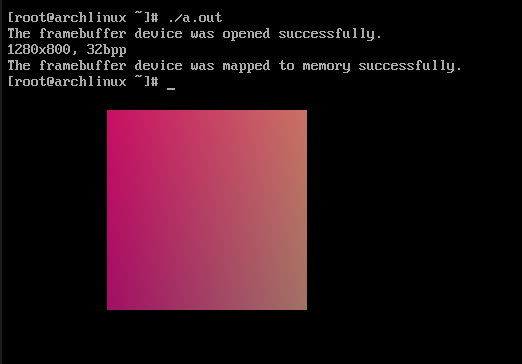
\includegraphics[scale=0.7]{realisierung/images/framebuffer-rectangle.png}
  \caption{C Programm welches einen Quadrat mit Gradient direkt in den Framebuffer schreibt}
\end{figure}

Jedoch wird es komplizierter, wenn man auch Text anzeigen möchte, da man jeden Pixel manuell schreiben muss welches bei Sätzen wie ``System Verification Failed'' bereits sehr umständlich ist.\\
Deshalb ist eine bessere lösung nötig, eine Bibliothek die in den Framebuffer schreiben kann und alle Rendering funktionen abstrahiert. Die Bibliothek die ich benutzt habe ist Raylib, eine C bibliothek welche hauptsächlich für die Entwicklung von Spielen gedacht ist, jedoch, nicht wie andere Engines, keine besonderen Features hat, sondern jediglich verschiedene Aspekte wie Grafik, Physik und Audio abstrahiert. Glücklicherweise kann mit der Compilerflag \texttt{-DEGL\_NO\_X11} raylib so kompiliert werden, dass es direkt in den Framebuffer schreibt, anstatt versucht ein Fenster zu öffnen.
\bigbreak \noindent
\begin{figure}[h]
  \centering
  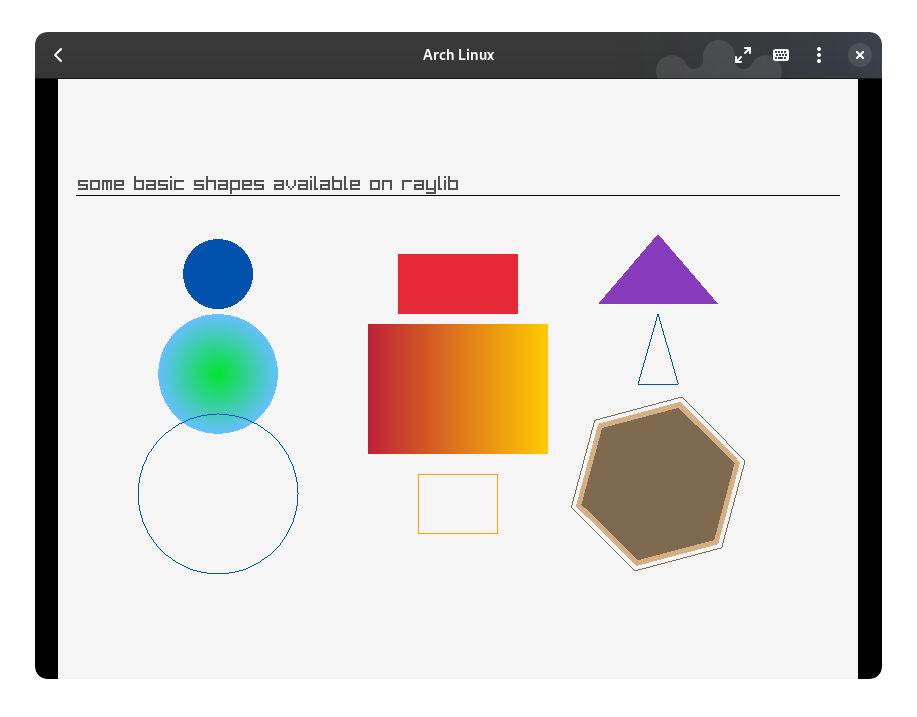
\includegraphics[scale=0.5]{realisierung/images/raylib-framebuffer.png}
  \caption{Raylib Beispielprogramm \texttt{shapes\_basic\_shapes} in einer VM mit output direkt zum Framebuffer}
\end{figure}

Hiermit wird es um einiges Einfacher eigene Bilder zu erstellen, die angezeigt werden wenn nötig.

\subsubsection{Grafikformat}
Da es recht umständlich wär, das Bild immer manuell in C zu programmieren, ist es am besten ein Grafikformat zu benutzen welches extern geladen werden kann. Der erste gedanke wäre, einfach jpg-xl oder png bilder zu benutzen, jedoch sind Rasterbasierte Grafikformate hier nicht sehr nützlich, da die Warnung auf viele verschiedene Bildschirmgrößen angezeigt werden muss, also sind Vektorbasierten Grafikformate nötig. Die bekannteste wäre SVG, eine XML basiertes Format mit dem Bilder geschrieben werden können, die unendlich groß skaliert werden können. SVG ist jedoch sehr komplex und hat features die hier nicht nötig sind.\\
Da ich kein Vektorbasiertes Grafikformat gefunden habe, welches auch sehr Simpel gehalten ist, habe ich mich entschlossen ein eigenes Format zu entwickeln.\\
\\
Das Format hat eine Funktionsbasierte Syntax, das heißt, dass im gegensatz zu SVG man einfach Funktionen aufruft um Formen zu zeichen oder Text zu schreiben:
\begin{verbatim}
rectangle (x=100,y=100,height=100,width=100,color="#FFFFFFFF",fill=true)
\end{verbatim}
Da diese art von Syntax sehr simpel zu Parsen ist, kann es alles direkt in POSIX-C implementiert werden, ohne externe Bibliotheken verwenden zu müssen.\\
Der nächste Schritt ist festzulegen, welche Funktionen benötigt werden. Mit betracht auf die Unterstützten Funktionen in raylib, habe ich die folgenden Funktionen implementiert:
\begin{itemize}
\item IMG\\
  Funktion um ein Bild zu Initialisieren, muss immer die erste Funktion in einem Bild sein.
\item rectangle\\
  Funktion um ein Rechteck zu zeichnen, unterstützt ausegfüllte und nicht ausgefüllte Rechtecke.
\item roundedrectangle\\
  Ein Rechteck aber mit abgerundeten Ecken.
\item circle\\
  Ein Kreis.
\item circlesegment\\
  Ein Kreissegment.
\item ring\\
  Ein Ring, kann genutzt werden um nicht ausegfüllte Kreise zu zeichnen.
\item ellipse\\
  Eine Ellipse.
\item triangle\\
  Ein Dreieck.
\item text\\
  Text.
\end{itemize}
Mit diesen Funktionen kann eine Bild ungefähr so aussehen:\\

\begin{verbatim}
// The IMG function is always required
// it initializes the image with its size
IMG (height=100, width=100)

// A rectangle 
rectangle (x=0, y=0, height=100, width=100, color="#5BCEFA", fill=true, thickness=0)

/*
 Rectangle but multiline
*/
rectangle (x=20, y=0,
height=60, width=100,
color="#F5A9B8",
fill=true, thickness=0)

circle (x=100,y=100,radius=10,color="#CfCfCf")
\end{verbatim}
Trotz des sehr simplen Aufbaus und kleinen Arsenal an Funktionen, ist es möglich viele verschiedene Dinge zu zeichnen, Perfekt um Grafiken für die Warnung von Nutzern zu erstellen.

\hypersetup{pageanchor=false}
\begin{figure}[h]
  \centering
  \begin{minipage}[c]{0.4\linewidth}
    
\includegraphics[width=\linewidth]{realisierung/images/bvg-haskell.png}
    \caption{Haskell Logo in bvg}
  \end{minipage}
  \hfill
  \begin{minipage}[c]{0.4\linewidth}
    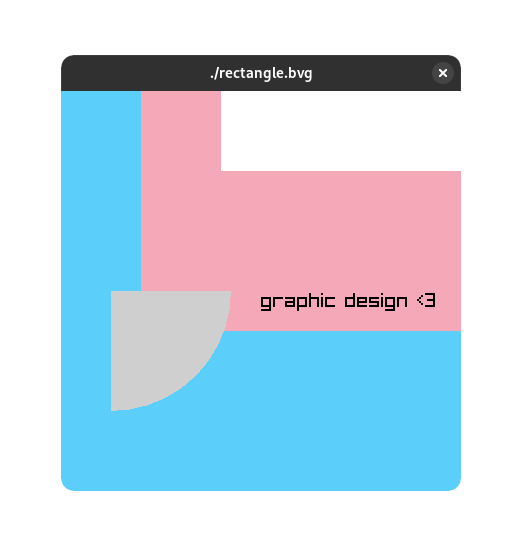
\includegraphics[width=\linewidth]{realisierung/images/bvg-rectangle.png}
    \caption{Rechtecke und Text}
  \end{minipage}
\end{figure}
\hypersetup{pageanchor=true}


%%% Local Variables:
%%% mode: LaTeX
%%% TeX-master: "../fsverify"
%%% End:
